\chapter{Physical Relational Operators}

One of the most important components in a DBMS is the \textbf{Query Manager}, which is responsible for scheduling queries and directing them to the correct tables. Part of the Query Manager is the \textbf{Query Optimizer}, which has the task of determining how to execute a query in the most efficient way possible, considering the physical parameters involved, the data organization, and the presence or absence of indexes.

This chapter will deal with how different physical operators are implemented, for the following operations:
\begin{itemize}
    \item Projection;
    \item Selection;
    \item Grouping;
    \item Set operations;
    \item Join.
\end{itemize}
Then, it will discuss how the optimizer uses these operators to generate efficient physical plans. In general, the problem will be studied under certain assumptions, illustrated in the next sections.

\section{Selectivity Factors}

The selectivity factor of a condition is an estimate of the percentage of the records in a relation which satisfy that condition. The simplest way to estimate this percentage is by assuming the data is uniformly distributed. The selectivity factor of different conditions in reported in table \ref{tab:sf-cond}. The last column is a constant value that is used if not enough information is known to calculate the actual $sf$, or when the attribute is non-numeric. 
\begin{table}[h]
\centering
\SetTblrInner{rowsep=5pt}
    \begin{tblr}{
        hlines,
        vlines,
        columns={145pt, c, m},
        column{1}={80pt}
    }
        Condition & Calculated $sf$ & Approx. $sf$ \\
    \hline
        $A = v$ & $\dfrac{1}{N_{key}}$ & $\dfrac{1}{10}$ \\
        $A > v$ & $\dfrac{\max(A) - v}{\max(A) - \min(A)}$ & $\dfrac{1}{3}$ \\
        $A < v$ & $\dfrac{v - \min(A)}{\max(A) - \min(A)}$ & $\dfrac{1}{3}$ \\
        $v_1 < A < v_2$ & $\dfrac{v_2 - v_1}{\max(A) - \min(A)}$ & $\dfrac{1}{4}$ \\
        $A_1 = A_2$ & $\dfrac{1}{\max(N_{key}(A), N_{key}(B))}$ & $\dfrac{1}{10}$ \\
        $\psi_1 \land \psi_2$ & $sf(\psi_1) \times sf(\psi_2)$ & - \\
        $\psi_1 \lor \psi_2$ & $sf(\psi_1) + sf(\psi_2) -$ $sf(\psi_1) \times sf(\psi_2)$ & - \\
    \end{tblr}
    \caption{Selectivity factors of different conditions.}
    \label{tab:sf-cond}
\end{table}

In many cases, however, attribute values follow non-uniform distributions, making these estimates wrong. The selectivity factor of a condition can be better approximated by knowing the actual distribution of the data, but storing the information needed to have full knowledge about it would occupy too much space. The solution preferred by DBMSs is to use a histogram with binned ranges of values in order to approximate the actual distribution.

There are two types of histograms: \textbf{equi-width} and \textbf{equi-height}. Equi-width histograms are obtained by binning values so that each bin has the same amount of elements $n$. For each bin, the sum of the counts of all elements inside that bin is stored. To find the selectivity factor for an equality search given a value $v$, it will be given by the sum associated with the bin $v$ belongs to, divided by $n$. For inequality/range searches, the selectivity factor will consider the sum associated with all the bins completely included in the range, plus the term that is given by the bin(s) corresponding to the extreme(s) of the condition.

The problem with equi-width histograms is that while they provide better approximations than a blind uniform distribution assumption, they are not able to correctly approximate the distribution of data to a sufficiently high precision. This is why equi-height histograms are used instead. These histograms are divided into bins such that the sum of counts of values within each (their ``height'') is equal across all of them. To store this type of histogram, the only information needed is the number of elements in each bin.

\begin{figure}[h]
    \centering
    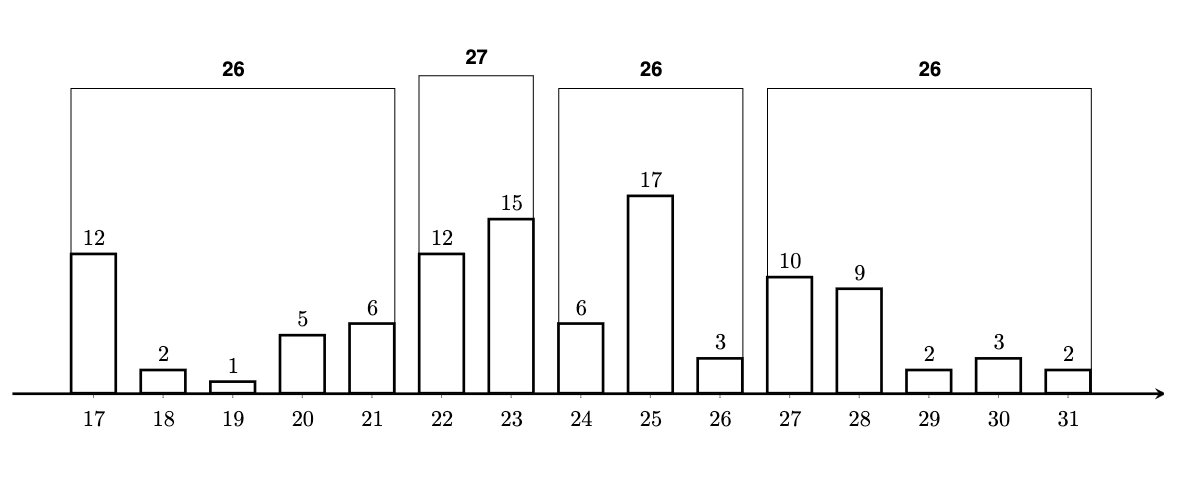
\includegraphics[width=0.7\linewidth]{img/equiheight.png}
    \caption{An equi-height histogram.}
    \label{fig:equi-height}
\end{figure}

Still, the approximation done by these histograms may not be accurate if the distribution within a bin is not uniform. For example, in Image \ref{fig:equi-height}, the third bin has follows a Gaussian distribution. If a query requests all records whose values for that attribute is equal to 24, the selectivity factor approximation will be much higher than the real one; if a query instead requests records with value 25, the approximation will be much lower.

\section{Physical Operators}

\subsection{Operators for Relation}

\paragraph{TableScan($R$)}
Returns all the records in $R$, in the same order as they are stores. It costs
\begin{equation*}
    C = N_{pag}(R)
\end{equation*}
The result size is
\begin{equation*}
    E_{rec} = N_{rec}(R)
\end{equation*}

\paragraph{SortScan($R, \{A_i\}$)}
Returns all the records in $R$ sorted in ascending order on the attribute $A_i$. Sorting is done with a merge sort algorithm. It costs
\begin{equation*}
    C = \begin{cases}
        N_{pag}(R) & N_{pag}(R) < B \\
        3 \times N_{pag}(R) & N_{pag}(R) \leq B \times (B-1) \\
        N_{pag}(R) + 2 \times N_{pag}(R) \times \ceil{log_{B-1}(N_{pag}(R) / B)} & \text{else}
    \end{cases}
\end{equation*}
The result size is
\begin{equation*}
    E_{rec} = N_{rec}(R)
\end{equation*}

\paragraph{IndexScan($R, I$)}
Returns the records of $R$ sorted by the attribute the index $I$ is defined on. It costs
\begin{equation*}
    C = \begin{cases}
        N_{leaf}(I) + N_{pag}(R) & \text{if $I$ is clustered} \\
        N_{leaf}(I) + N_{rec}(R) & \text{if $I$ is on a key of $R$} \\
        N_{leaf}(I) + \ceil{N_{key}(I) \times \phi(\ceil{N_{rec}(R) / N_{key}(I)}, N_{pag}(R))} & \text{else}
    \end{cases}
\end{equation*}
The result size is
\begin{equation*}
    E_{rec} = N_{rec}(R)
\end{equation*}

\paragraph{IndexSequentialScan($R, I$)}
Returns the records of $R$, stored with the primary organization index sequential file $I$, sorted in ascending order on the primary key values. It costs
\begin{equation}
    C = N_{leaf}(I)
\end{equation}
The result size is
\begin{equation*}
    E_{rec} = N_{rec}(R)
\end{equation*}

\subsection{Operators for Projection}

\paragraph{Project($O, \{A_i\}$)}
Projects the records of $O$ over the attributes $\{A_i\}$. It costs
\begin{equation*}
    C = C(O)
\end{equation*}
The result size is
\begin{equation*}
    E_{rec} = E_{rec}(O)
\end{equation*}

\paragraph{IndexOnlyScan($R, I, \{A_i\}$)}
Returns the sorted records of $R$, projecting them over the attributes $\{A_i\}$ on which the index $I$ is on (or contains them as prefix). It costs
\begin{equation*}
    C = N_{leaf}(I)
\end{equation*}
If a tuple of values for the attributes $\{A_i\}$ is associated with $n$ different RIDs, it is returned $n$ times. The result will not contain duplicates if the attributes are relation keys (they uniquely identify records). The result size is
\begin{equation*}
    E_{rec} = N_{rec}(R)
\end{equation*}

\subsection{Operators for Duplicate Elimination}

\paragraph{Distinct($O$)}
Returns the records of $O$ eliminating all duplicates. This operator requires that the records of $O$ are \textbf{grouped} (if $r_i = r_j$, and $i < l < j$, then $r_i = r_l = r_j$). When a collection of records is sorted, it is also grouped. It costs
\begin{equation*}
    C = C(O)
\end{equation*}
If there's only one attribute in $O$, then the result size is
\begin{equation*}
    E_{rec} = N_{key}(A)
\end{equation*}
If instead it contains multiple attributes, the result size is
\begin{equation*}
    E_{rec} = \min(|O|/2, \prod_i N_{key}(A_i))
\end{equation*}
This is a pessimistic estimate: it assumes that there is a record for each set of values taken from the attributes in $O$, but this is often not the actual result. For example, imagine a database containing data about students enrolled at a university, and the two attributes represent their first name and last name respectively: it is unrealistic to expect that there will be a different student for each first name-last name combination, even if the two attributes are loosely correlated.

\paragraph{HashDistinct($O$)}
Returns the records of $O$ without duplicates using and hash technique. This technique has two phases: \textbf{partitioning} and \textbf{duplicate elimination}. Assume the query processor has $B+1$ buffer pages. In the partitioning phase, for each record in $O$ the hash function $h_1$ is applied, distributing records uniformly across the $B$ pages. Once a page $i$ is full, it is written to the $T_i$ partition file. At the end of the phase, all records will be scattered across $B$ files, each of which contains records with the same hash value; this means that duplicates are found in the same partition.

In the duplicate elimination phase, the process becomes an intra-partition problem. Each $T_i$ file is read page-by-page, eliminating duplicates using the hash function $h_2$. A record is deleted when it collides with another record with the same hash value according to $h_2$ and the two records are identical. Assuming each partition occupies at most $B$ pages, at the end of the partition, the $B$ pages are cleared, and the duplicate elimination is applied to the records in the next partition. If the number of pages is greater than $B$, then a hash-based projection technique is applied recursively by dividing the partition into subpartitions. This degrades performances. The operator costs:
\begin{equation*}
    C = C(O) + 2 \times N_{pag}(O)
\end{equation*}
The result size is the same as Distinct, so
\begin{equation*}
    E_{rec} = N_{key}(A)
\end{equation*}
if there's only one attribute in $O$, and
\begin{equation*}
    E_{rec} = \min(|O|/2, \prod_i N_{key}(A_i))
\end{equation*}
if $O$ contains multiple attributes.

\subsection{Operators for Sort}

\paragraph{Sort($O, \{A_i\}$)}
Returns the records of $O$ sorted on the attributes $\{A_i\}$. The sorting algorithm used is merge-sort, so its cost is
\begin{equation*}
    C = \begin{cases}
        C(O) & N_{pag}(O) < B \\
        C(O) + 2 \times N_{pag}(O) & N_{pag}(O) \leq B \times (B-1) \\
        C(O) + 2 \times N_{pag}(O) \times \ceil{log_{B-1}(N_{pag}(O) / B)} & \text{else}
    \end{cases}
\end{equation*}
The result size is
\begin{equation*}
    E_{rec} = N_{rec}(O)
\end{equation*}

\subsection{Operators for Selection}

\paragraph{Filter($O,\psi$)}
Returns the records of $O$ that satisfy the condition $\psi$. It costs
\begin{equation*}
    C = C(O)
\end{equation*}
The result size is
\begin{equation*}
    \ceil{sf(\psi) \times N_{rec}(O)}
\end{equation*}

\paragraph{IndexFilter($R,I,\psi$)}
Returns the records of $R$ that satisfy the condition $\psi$ using the index $I$, defined on the attributes involved in $\psi$, sorted according to $I$. The condition is a predicate or a conjunction of predicates that only involve the attributes found in the prefix of the index search key.

IndexFilter always appears as a leaf node in a physical plan. This operator uses the index to find the sorted set of RIDs of all records that satisfy the condition, then it retrieves the records from disk. The cost can be broken down as
\begin{equation*}
    C = C_I + C_D
\end{equation*}
\begin{itemize}
    \item If the index is clustered:
    \begin{align*}
        &C_I = \ceil{sf(\psi) \times N_{leaf}(I)} \\
        &C_D = \ceil{sf(\psi) \times N_{pag}(R)}
    \end{align*}

    \item If the index is unclustered:
    \begin{align*}
        &C_I = \ceil{sf(\psi) \times N_{leaf}(I)} \\
        &C_D = \ceil{sf(\psi) \times N_{key}(I)} \times \ceil{\Phi(\ceil{N_{rec}(R) / N_{key}(I)}, N_{pag}(R))}
    \end{align*}
    If the index is defined on a key of $R$, then
    \begin{equation*}
        C_D = \ceil{sf(\psi) \times N_{rec}(R)}
    \end{equation*}
\end{itemize}
The result size is
\begin{equation*}
    E_{rec} = \ceil{sf(\psi) \times N_{rec}(R)}
\end{equation*}

\paragraph{IndexSequentialFilter($R,I,\psi$)}
Returns the sorted records of $R$, stored with the primary organization index sequential file $I$, satisfying the condition $\psi$, which involves only the attributes of the index search key. It costs
\begin{equation*}
    C = \ceil{sf(\psi) \times N_{leaf}(I)}
\end{equation*}
The result size is
\begin{equation*}
    E_{rec} = \ceil{sf(\psi) \times N_{rec}(R)}
\end{equation*}

\paragraph{IndexOnlyFilter($R, I, \{A_i\}, \psi$)}
Returns the sorted records of the projection on $R$ returning only the values for $\{A_i\}$ that satisfy $\psi$, using only the index $I$. It costs
\begin{equation*}
    C = \ceil{sf(\psi) \times N_{leaf}(I)}
\end{equation*}
The result size is
\begin{equation*}
    E_{rec} = \ceil{sf(\psi) \times N_{rec}(R)}
\end{equation*}

\subsection{Operators for Grouping}

\paragraph{GroupBy($O, \{A_i\}, \{f_i\}$)}
Returns the records of $O$ sorted on $\{A_i\}$, applying the aggregation functions $\{f_i\}$. The records in $O$ must already be sorted beforehand. It costs
\begin{equation*}
    C = C(O)
\end{equation*}

\paragraph{HashGroupBy($O, \{A_i\}, \{f_i\}$)}
Returns the records of $O$ grouped by $\{A_i\}$, applying the aggregation functions $\{f_i\}$. The records are not sorted on $\{A_i\}$. The grouping is done using two phases, like HashDistinct. In the first phase, called partitioning phase, a partition is created using the hash function $h_1$; in the second phase, called grouping, the records of each partition are grouped using the hash function $h_2$ applied to all grouping attributes. When two records with the same grouping attributes are found, a step to compute the aggregate function is applied. The operator costs
\begin{equation*}
    C = C(O) + 2 \times N_{pag}(O)
\end{equation*}

For both the previous two operators, the result size is calculated as for the duplicate elimination. If there's only one attribute in $O$, then the result size is
\begin{equation*}
    E_{rec} = N_{key}(A)
\end{equation*}
If instead it contains multiple attributes, the result size is
\begin{equation*}
    E_{rec} = \min(|O|/2, \prod_i N_{key}(A_i))
\end{equation*}

\subsection{Operators for Join}

\paragraph{NestedLoop($O_E, O_I, \psi_J$)}
Joins the external operand $O_E$ with the internal operand $O_I$ with the following algorithm:
\begin{algorithm}
\begin{algorithmic}
    \For{$r \in O_E$}
        \For{$s \in O_I$}
            \State If $\psi_J$, add $<r,s>$ to the result.
        \EndFor
    \EndFor
\end{algorithmic}
\end{algorithm} \\
It costs
\begin{equation*}
    C = C(O_E) + E_{rec}(O_E) \times C(O_I)
\end{equation*}
The result size is
\begin{equation*}
    E_{rec} = sf(\psi_j) \times E_{rec}(O_E) \times E_{rec}(O_I)
\end{equation*}

\paragraph{PageNestedLoop($O_E, O_I, \psi_J$)}
Joins the external operand with the internal operand by scanning $O_I$ once per page of $O_E$ (and not once per record, as for NestedLoop). The algorithm used is the following:
\begin{algorithm}
\begin{algorithmic}
    \For{$p_r$ of $O_E$}
        \For{$p_s$ of $O_I$}
            \For{$r \in p_r$}
                \For{$s \in p_s$}
                    \State If $\psi_J$, add $<r,s>$ to the result. 
                \EndFor
            \EndFor
        \EndFor
    \EndFor
\end{algorithmic}
\end{algorithm} \\
The cost of the operator is
\begin{equation*}
    C = C(O_E) + N_{pag}(O_E) \times C(O_I)
\end{equation*}
The algorithm cost is lower when the external operand is the one with fewer pages.
The result size is
\begin{equation*}
    E_{rec} = sf(\psi_j) \times E_{rec}(O_E) \times E_{rec}(O_I)
\end{equation*}

\paragraph{BlockNestedLoop($O_E, O_I, \psi_J$)}
Joins the external operand $O_E$ with the internal operand $O_I$ by extending PageNestedLoop using more memory for a group of pages of the external operand. Assume the operands are TableScan of tables $R$ and $S$, and that the query processor has $B+2$ pages in the buffer. $B$ pages are used for the external operand, 1 page for an input page of $S$, and 1 page is reserved as the output buffer. For each record $r$ of a page group of $R$, and for each joining record $s$ of a page in $S$, $<r,s>$ is written to the output buffer page.

The cost of the operator is
\begin{equation*}
    C = N_{pag}(R) + \ceil{N_{pag}(R)/B} \times N_{pag}(S)
\end{equation*}
The cost is lower if the external relation has fewer pages than the internal one. If the $B$ pages are enough to contain one of the two relations, then the cost is reduced to
\begin{equation*}
    N_{pag}(R) + N_{pag}(S)
\end{equation*}
The result size is
\begin{equation*}
    E_{rec} = sf(\psi_j) \times E_{rec}(O_E) \times E_{rec}(O_I)
\end{equation*}
This operator is not convenient to use when the operators require too many pages (i.e., $N_{pag}R \geq B^2$).

\paragraph{IndexNestedLoop($O_E, O_I, \psi_J$)}
This operator requires that there is an index on the join column of the internal operand, and performs a join with the following algorithm:
\begin{algorithm}
\begin{algorithmic}
    \For{$r \in O_E$}
        \For{$s \in$ IndexFilter($O_I, I, O_E.e1 = O_I.i1$)}
            \State Add $<r,s>$ to the result.
        \EndFor
    \EndFor
\end{algorithmic}
\end{algorithm} \\
It costs
\begin{equation*}
    C = C(O_E) + E_{rec}(O_E) \times (C_I + C_D)
\end{equation*}
where $C_I$ and $C_D$ are the costs to retrieve the relevant index records and the data from disk. If the internal operand is an IndexFilter($S,I,\psi_J$), the result size is
\begin{equation*}
    E_{rec} = \ceil{sf(\psi_J) \times E_{rec}(O_E) \times N_{rec}(S)}
\end{equation*}
if instead it is a Filter(IndexFilter($S, I, \psi_J$), $\psi$), the result size is
\begin{equation*}
    E_{rec} = \ceil{sf(\psi_J) \times E_{rec}(O_E) \times (sf(\psi) \times N_{rec}(S))}
\end{equation*}

\paragraph{MergeJoin($O_E, O_I, \psi_J$)}
This operator requires that $O_E$ and $O_I$ are sorted on the same join attributes, and that in the join condition, $O_E.A_i$ is a key of $O_E$. Since this join attribute has distinct values in $O_E$, the algorithm reads the records of $O_E$ one by one, and reads all records of $O_I$ with the same values (which will be found one after the other). This operator costs
\begin{equation*}
    C = C(O_E) + C(O_I)
\end{equation*}
The result size is
\begin{equation*}
    E_{rec} = \ceil{sf(\psi_J) \times E_{rec}(O_E) \times E_{rec}(O_I)}
\end{equation*}

\paragraph{HashJoin($O_E, O_I, \psi_J$)}
Returns the join result with a hash technique in two phases. In the first phase, called partitioning phase, the records of both operands are partitioned using the hash function $h_1$, similarly to HashDistinct. In the second phase, called \textbf{probing} (or \textbf{matching}), for each $B_i$ partition, the records of $O_E$ are read and inserted into the buffer hash table with $B$ pages using the hash function $h_2$. The records of $O_I$ are read one page at a time, $h_2$ is applied to them, and if there is a match with the records in $O_E$, the joined record is added to the result.

Assuming $N_{pag}(O_E)/B < B$ and that the pages are uniform, the cost of the operator is
\begin{equation*}
    C = C(O_E) + C(O_I) + 2 \times (N_{pag}(O_E) + N_{pag}(O_I))
\end{equation*}
where $(C(O_E) + C(O_I) + (N_{pag}(O_E) + N_{pag}(O_I))$ is the cost of the partitioning phase, and $(N_{pag}(O_E) + N_{pag}(O_I))$ is the cost of the probing phase. However, if the pages are not uniform, the resulting partitions will not have the same size, they may not fit in $B$. The cost can be generalized to
\begin{equation*}
    C = (\log_B(N_{pag}(O_E)) \times 2 - 2) \times (N_{pag}(O_E) + N_{pag}(O_I))
\end{equation*}
If $N_{pag}(O_E) < B$, the cost is 0.

The result size is
\begin{equation*}
    E_{rec} = \ceil{sf(\psi_J) \times E_{rec}(O_E) \times E_{rec}(O_I)}
\end{equation*}